\documentclass[a4paper]{article}

\usepackage[english]{babel}
\usepackage[utf8x]{inputenc}
\usepackage{amsmath}
\usepackage{graphicx}
\usepackage[colorinlistoftodos]{todonotes}
\usepackage{dsfont}
\usepackage{upgreek}
\usepackage{tikz}

\title{ALGEBRA III}
\author{Sergio Padilla López}

\begin{document}
\maketitle

\section{Ejercicio 1}

Se considera la ecuación $x^{4}-3=0$, con raices $\sqrt[4]{3}, i\sqrt[4]{3}, -\sqrt[4]{3} y -i\sqrt[4]{3}$. Estas generan el cuerpo $\mathds{Q}(\sqrt[4]{3},i) $ sobre $\mathds{Q}$.Cada automorfismo de $\mathds{Q}(\sqrt[4]{3},i)/\mathds{Q}$ envia $\sqrt[4]{3}$ a una de las raices de $x^{4}-3=0$ y envía i a una de las raices de $x^{2}+1=0$. Por tanto como máximo tenemos ocho automorfismos, que forman un grupo, y que están generados por $\varphi(i)=-i $, $\varphi(\sqrt[4]{3})=\sqrt[4]{3}$ y $\psi(i)=i $, $\psi(\sqrt[4]{3})=i\sqrt[4]{3}$.

\begin{enumerate}
\item Prueba que $\langle\varphi,\psi\rangle$ = Aut($\mathds{Q}(\sqrt[4]{3},i)/\mathds{Q}$) el grupo de todos los automorfismos de la extensión $\mathds{Q}(\sqrt[4]{3},i)$ es isomorfo a $D_{4}$, identificando $\varphi$ y $\psi$ con simetrías del cuadrado. En este caso, $\psi$ es el giro de amplitud $\frac{\pi}{4}$ y $\varphi$ es la simetría del eje (1-3).

\item Representa por permutaciones los elementos de $\varphi$ y $\psi$.

\item Dibuja el retículo de subgrupos de $D_{4}$ con notación de permutaciones y en función de $\varphi$ y $\psi$.

\item Observa que tiene exactamente tres subgrupos de orden 4, y cinco subgrupos de orden 2.
\end{enumerate}
\

\textbf{SOLUCIÓN}

\begin{enumerate}
\item Vamos a probarlo comprobando que se verifican las igualdades características de $D_{4}$:
\begin{equation}\label{eq:a}
s^2=1
\end{equation}
\begin{equation}\label{eq:b}
r^4=1
\end{equation}
\begin{equation}\label{eq:c}
sr=r^{3}s
\end{equation}
Tomamos $\varphi = s$ y veamos que cumple $\varphi^{2}$ es la identidad:
\begin{equation*}
\varphi^{2}(i)=\varphi(\varphi(i))=\varphi(-i)=-(-i)=i
\end{equation*}
\begin{equation*}
\varphi^{2}(\sqrt[4]{3})=\varphi(\varphi(\sqrt[4]{3}))=\varphi(\sqrt[4]{3})=\sqrt[4]{3}
\end{equation*}

Sea ahora $\psi = r$ veamos que $\psi^{4}$ es la identidad:
\begin{equation*}
\psi^{4}(i)=\psi^{3}(\psi(i))=\psi^{3}(i)=\psi^{2}(\psi(i))=\psi^{2}(i)=\psi(\psi(i))=\psi(i)=i
\end{equation*}
\begin{equation*}
\psi^{4}(\sqrt[4]{3})=\psi^{3}(\psi(\sqrt[4]{3}))=\psi^{3}(i\sqrt[4]{3})=\psi^{2}(i^{2}\sqrt[4]{3})=\psi(i^{3}\sqrt[4]{3})=i^{4}\sqrt[4]{3}=\sqrt[4]{3}
\end{equation*}

Por último, veamos que se verifica \ref{eq:c}:
\begin{equation*}
\varphi\psi(i)=\varphi(i)=-i=\psi(-i)=\psi^{2}(-i)=\psi^{3}(-i)=\psi^{3}\varphi(i)
\end{equation*}

\item \{1,(24),(1234),(14)(23),(13),(13)(24),(1432),(12)(34)\}
\

%%%%%%%%%%%%%%%%%
% RETICULO DE D4
%%%%%%%%%%%%%%%%%
\item
\

\begin{center}
\begin{tikzpicture}[scale=0.2]
\tikzstyle{every node}+=[inner sep=0pt]
\draw (39.3,-6.5) node {$D_4$};
\draw (38.9,-20) node {$\langle\psi\rangle$};
\draw (58.2,-18.8) node {$\langle\varphi,\psi^{2}\rangle$};
\draw (22.6,-18.8) node {$\langle\psi^{2},\varphi\psi\rangle$};
\draw (53.7,-33.3) node {$\langle\varphi\rangle$};
\draw (25.8,-33.3) node {$\langle\varphi\psi\rangle$};
\draw (38.9,-33.3) node {$\langle\psi^{2}\rangle$};
\draw (12.5,-33.3) node {$\langle\varphi\psi^{3}\rangle$};
\draw (68.1,-33.3) node {$\langle\varphi\psi^{2}\rangle$};
\draw (38.9,-48.8) node {$1$};
\draw [black] (38.99,-17) -- (39.21,-9.5);
\fill [black] (39.21,-9.5) -- (38.69,-10.28) -- (39.69,-10.31);
\draw [black] (55.69,-17.16) -- (41.81,-8.14);
\fill [black] (41.81,-8.14) -- (42.21,-8.99) -- (42.76,-8.15);
\draw [black] (25.02,-17.02) -- (36.88,-8.28);
\fill [black] (36.88,-8.28) -- (35.94,-8.35) -- (36.54,-9.16);
\draw [black] (40.97,-46.63) -- (51.63,-35.47);
\fill [black] (51.63,-35.47) -- (50.71,-35.7) -- (51.44,-36.39);
\draw [black] (36.96,-46.51) -- (27.74,-35.59);
\fill [black] (27.74,-35.59) -- (27.87,-36.53) -- (28.63,-35.88);
\draw [black] (38.9,-45.8) -- (38.9,-36.3);
\fill [black] (38.9,-36.3) -- (38.4,-37.1) -- (39.4,-37.1);
\draw [black] (36.31,-47.28) -- (15.09,-34.82);
\fill [black] (15.09,-34.82) -- (15.52,-35.66) -- (16.03,-34.79);
\draw [black] (41.55,-47.39) -- (65.45,-34.71);
\fill [black] (65.45,-34.71) -- (64.51,-34.64) -- (64.98,-35.52);
\draw [black] (36.66,-31.31) -- (24.84,-20.79);
\fill [black] (24.84,-20.79) -- (25.11,-21.7) -- (25.77,-20.95);
\draw [black] (41.3,-31.5) -- (55.8,-20.6);
\fill [black] (55.8,-20.6) -- (54.86,-20.68) -- (55.46,-21.48);
\draw [black] (38.9,-30.3) -- (38.9,-23);
\fill [black] (38.9,-23) -- (38.4,-23.8) -- (39.4,-23.8);
\draw [black] (14.21,-30.84) -- (20.89,-21.26);
\fill [black] (20.89,-21.26) -- (20.02,-21.63) -- (20.84,-22.2);
\draw [black] (66.41,-30.82) -- (59.89,-21.28);
\fill [black] (59.89,-21.28) -- (59.93,-22.22) -- (60.76,-21.66);
\draw [black] (54.59,-30.43) -- (57.31,-21.67);
\fill [black] (57.31,-21.67) -- (56.6,-22.28) -- (57.55,-22.58);
\draw [black] (25.15,-30.37) -- (23.25,-21.73);
\fill [black] (23.25,-21.73) -- (22.93,-22.62) -- (23.91,-22.4);
\end{tikzpicture}
\end{center}


%%%%%%%%%%%%%%%%%%

%%%%%%%%%%%%%%%%%
% RETICULO DE D4
%%%%%%%%%%%%%%%%%

\

\begin{center}
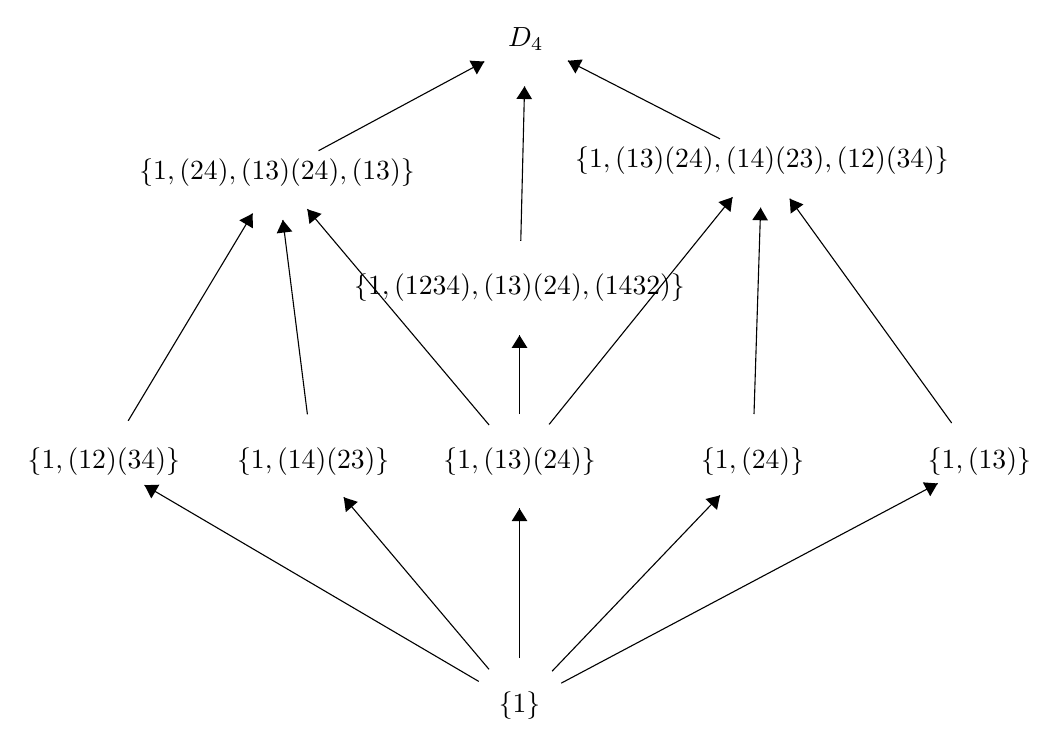
\begin{tikzpicture}[scale=0.2]
\tikzstyle{every node}+=[inner sep=0pt]
\draw (39.3,-6.5) node {$D_4$};
\draw (38.9,-22.3) node {$\{1,(1234),(13)(24),(1432)\}$};
\draw (54.3,-14.2) node {$\{1,(13)(24),(14)(23),(12)(34)\}$};
\draw (23.5,-15) node {$\{1,(24),(13)(24),(13)\}$};
\draw (53.7,-33.3) node {$\{1,(24)\}$};
\draw (25.8,-33.3) node {$\{1,(14)(23)\}$};
\draw (38.9,-33.3) node {$\{1,(13)(24)\}$};
\draw (12.5,-33.3) node {$\{1,(12)(34)\}$};
\draw (68.1,-33.3) node {$\{1,(13)\}$};
\draw (38.9,-48.8) node {$\{1\}$};
\draw [black] (38.98,-19.3) -- (39.22,-9.5);
\fill [black] (39.22,-9.5) -- (38.7,-10.29) -- (39.7,-10.31);
\draw [black] (51.63,-12.83) -- (41.97,-7.87);
\fill [black] (41.97,-7.87) -- (42.45,-8.68) -- (42.91,-7.79);
\draw [black] (26.14,-13.58) -- (36.66,-7.92);
\fill [black] (36.66,-7.92) -- (35.72,-7.86) -- (36.19,-8.74);
\draw [black] (40.97,-46.63) -- (51.63,-35.47);
\fill [black] (51.63,-35.47) -- (50.71,-35.7) -- (51.44,-36.39);
\draw [black] (36.96,-46.51) -- (27.74,-35.59);
\fill [black] (27.74,-35.59) -- (27.87,-36.53) -- (28.63,-35.88);
\draw [black] (38.9,-45.8) -- (38.9,-36.3);
\fill [black] (38.9,-36.3) -- (38.4,-37.1) -- (39.4,-37.1);
\draw [black] (36.31,-47.28) -- (15.09,-34.82);
\fill [black] (15.09,-34.82) -- (15.52,-35.66) -- (16.03,-34.79);
\draw [black] (41.55,-47.39) -- (65.45,-34.71);
\fill [black] (65.45,-34.71) -- (64.51,-34.64) -- (64.98,-35.52);
\draw [black] (36.97,-31) -- (25.43,-17.3);
\fill [black] (25.43,-17.3) -- (25.56,-18.23) -- (26.33,-17.59);
\draw [black] (40.78,-30.96) -- (52.42,-16.54);
\fill [black] (52.42,-16.54) -- (51.53,-16.84) -- (52.3,-17.47);
\draw [black] (38.9,-30.3) -- (38.9,-25.3);
\fill [black] (38.9,-25.3) -- (38.4,-26.1) -- (39.4,-26.1);
\draw [black] (14.05,-30.73) -- (21.95,-17.57);
\fill [black] (21.95,-17.57) -- (21.11,-18) -- (21.97,-18.51);
\draw [black] (66.34,-30.87) -- (56.06,-16.63);
\fill [black] (56.06,-16.63) -- (56.12,-17.57) -- (56.93,-16.99);
\draw [black] (53.79,-30.3) -- (54.21,-17.2);
\fill [black] (54.21,-17.2) -- (53.68,-17.98) -- (54.68,-18.01);
\draw [black] (25.43,-30.32) -- (23.87,-17.98);
\fill [black] (23.87,-17.98) -- (23.48,-18.83) -- (24.47,-18.71);
\end{tikzpicture}
\end{center}
%%%%%%%%%%%%%%%%%%%%%

\end{enumerate}

\section{Ejercicio 2}
Dada la extensión de cuerpos $\mathds Q(\sqrt[4]3, i)/\mathds Q$, ya que tenemos la siguiente torre de cuerpos: $\mathds Q \subset \mathds Q(\sqrt[4]3) \subset \mathds Q(\sqrt[4]3, i)$, tenemos una base de $\mathds Q(\sqrt[4]3, i)$ sobre $\mathds Q$ que tiene ocho elementos, y cada elemento $x\in \mathds Q(\sqrt[4]3, i)$ se escribe de forma única como
\begin{equation*}
 x = a_0 + a_1\sqrt[4]3 + a_2{\sqrt[4]3}^2 + a_3{\sqrt[4]3}^3 + a_4 i + a_5 i\sqrt[4]3 + a_6 i{\sqrt[4]3}^2 + a_7 i{\sqrt[4]3}^3
\end{equation*}

Observa que si se considera el subgrupo $\left<\psi\right>$, los elementos que quedan fijos para $\psi$ son exactamente
los que quedan fijos para cada elemento del subgrupo que $\psi$ genera.

\begin{enumerate}
\item Prueba que si se considera un subgrupo $H=\left<\phi_1,\dots,\phi_t\right>\subset\mathrm{Aut}(\mathds Q(\sqrt[4]3, i)/\mathds Q)$, un elemento $x$ queda fijo para todos los elementos de $H$ si, y solo si, queda fijo para $\phi_1,\dots,\phi_t$.
\item Prueba que el conjunto de los elementos $x$ que quedan fijos para un subgrupo $H$ es un cuerpo, al que llamaremos $F^H$, y que verifica $\mathds Q\subset F^H\subset\mathds Q(\sqrt[4]3,i)$.
\item Prueba que si $H_1\subset H_2\subset \mathrm{Aut}(\mathds Q(\sqrt[4]3, i)/\mathds Q)$ son subgrupos, entonces $F^{H_2}\subset F^{H_1}$.
\item Dibuja el retículo de los subcuerpos $F^H$, donde $H$ varía entre los subgrupos de $\mathrm{Aut}(\mathds Q(\sqrt[4]3, i)/\mathds Q)$.
\end{enumerate}
\

\textbf{SOLUCIÓN}

\begin{enumerate}
\item Veamos la implicación de izquierda a derecha. Basta con saber como son los elementos de $H$, que son los propios $\phi_1,\dots,\phi_t$ y composiciones de estos mismos. Luego es claro que si $x$ queda fijo para todos los elementos de $H$, en particular, tiene que quedar fijo para $\phi_1,\dots,\phi_t$.

Veamos la implicación de derecha a izquierda. Si $x$ queda fijo para $\phi_1,\dots,\phi_t$, tenemos que para todo elemento de $H$, al ser composición de elementos de $\phi_1,\dots,\phi_t$, se conserva por composición, luego $x$ queda fijo para todo elemento de $H$.

\item Para ello, teniendo en cuenta que un elemento de $H$ es un automorfismo, vamos a probar que es cerrado para la suma y el producto. Sea $x$,$y \in F^H$ y sea $\varphi \in H$ cualquiera:
\begin{equation*}
\varphi(x+y)=\varphi(x)+\varphi(y)=x+y
\end{equation*}
\begin{equation*}
\varphi(x \times y)=\varphi(x) \times \varphi(y)=x\times y
\end{equation*}

\item Sea $x \in F^{H_2}$ cualquiera, por definición, $x$ es fijo para todos los elementos de $H_2$. Como $H_1 \subset H_2$, $\forall \varphi \in H_1, \varphi \in H_2$ luego si $x$ es fijo para todos los elementos de $H_2$, en particular es fijo para todos los elementos de $H_1$, y por tanto, $F^{H_2}\subset F^{H_1}$.

\newpage

\item \


\begin{center}
\begin{tikzpicture}[scale=0.2]
\tikzstyle{every node}+=[inner sep=0pt]
\draw (38.9,-5.1) node {$\{1\}$};
\draw (24.7,-20.1) node {$F^{\langle\varphi\psi}\rangle$};
\draw (38.9,-20.1) node {$F^{\langle\psi^{2}}\rangle$};
\draw (10.4,-20.1) node {$F^{\langle\varphi\psi^{3}}\rangle$};
\draw (38.9,-35.7) node {$F^{\langle\psi\rangle}$};
\draw (70.4,-20.1) node {$F^{\langle\varphi\psi^{2}}\rangle$};
\draw (20.7,-35.7) node {$F^{\langle\psi^{2},\varphi\psi\rangle}$};
\draw (55.5,-20.1) node {$F^{\langle\varphi\rangle}$};
\draw (60,-35.7) node {$F^{\langle\varphi\psi^{2}\rangle}$};
\draw (38.9,-50.6) node {$F^{\langle\varphi,\psi\rangle}$};
\draw [black] (41.35,-48.87) -- (57.55,-37.43);
\fill [black] (57.55,-37.43) -- (56.61,-37.48) -- (57.18,-38.3);
\draw [black] (38.9,-47.6) -- (38.9,-38.7);
\fill [black] (38.9,-38.7) -- (38.4,-39.5) -- (39.4,-39.5);
\draw [black] (36.55,-48.74) -- (22.45,-37.56);
\fill [black] (22.45,-37.56) -- (22.77,-38.45) -- (23.39,-37.67);
\draw [black] (18.52,-33.15) -- (11.98,-22.65);
\fill [black] (11.98,-22.65) -- (11.98,-23.59) -- (12.83,-23.06);
\draw [black] (20.95,-32.82) -- (23.85,-22.98);
\fill [black] (23.85,-22.98) -- (23.15,-23.6) -- (24.1,-23.89);
\draw [black] (38.9,-32.7) -- (38.9,-23.1);
\fill [black] (38.9,-23.1) -- (38.4,-23.9) -- (39.4,-23.9);
\draw [black] (61.66,-33.2) -- (68.74,-22.6);
\fill [black] (68.74,-22.6) -- (67.88,-22.98) -- (68.71,-23.54);
\draw [black] (59.17,-32.82) -- (56.33,-22.98);
\fill [black] (56.33,-22.98) -- (56.07,-23.89) -- (57.03,-23.61);
\draw [black] (13.05,-18.7) -- (36.25,-6.5);
\fill [black] (36.25,-6.5) -- (35.3,-6.43) -- (35.77,-7.31);
\draw [black] (26.76,-17.92) -- (36.84,-7.28);
\fill [black] (36.84,-7.28) -- (35.92,-7.52) -- (36.65,-8.2);
\draw [black] (38.9,-17.1) -- (38.9,-8.1);
\fill [black] (38.9,-8.1) -- (38.4,-8.9) -- (39.4,-8.9);
\draw [black] (53.27,-18.09) -- (41.13,-7.11);
\fill [black] (41.13,-7.11) -- (41.38,-8.02) -- (42.05,-7.28);
\draw [black] (67.69,-18.81) -- (41.61,-6.39);
\fill [black] (41.61,-6.39) -- (42.12,-7.19) -- (42.55,-6.28);
\draw [black] (22.41,-33.78) -- (36.59,-22.02);
\fill [black] (36.59,-22.02) -- (35.66,-22.14) -- (36.29,-22.91);
\draw [black] (57.59,-33.92) -- (41.31,-21.88);
\fill [black] (41.31,-21.88) -- (41.66,-22.76) -- (42.25,-21.96);
\end{tikzpicture}
\end{center}
\end{enumerate}

\section{Ejercicio 3}
Escribir, en función de los polinomios simétricos elementales en $X,Y,Z$, el polinomio $p(X,Y,Z) = X^4 +Y^4 +Z^4 \in \mathds{Q}[X,Y,Z]$. Detallar, paso a paso, la aplicación del algoritmo.
\\

\textbf{SOLUCIÓN}
\\

Vamos a utilizar el método de los coeficientes indeterminados. Como sabemos $p$ puede escribirse de forma única en función de los polinomios $e_i$ con coeficientes en $\mathds{Q}$. Como $p$ es un polinomio simétrico, homogeneo y de grado 4, voy a considerar los polinomios de grado 4 que puedo formar con polinomios simétricos elementales, y considero la siguiente combinación lineal:
\begin{equation*}
p = \alpha e_1^4 + \beta e_2^2 + \gamma e_3e_1 + \delta e_1^2e_2
\end{equation*}

La expresión anterior es una igualdad de polinomios en $X,Y,Z$, luego se conserva al evaluar $X,Y,Z$. Por tanto, vamos a dar valores aleatorios a las variables para obtener igualdades de donde podamos despejar los coeficientes $\alpha,\beta,\gamma$ y $\delta$.

\begin{equation*}
X=1, Y=Z=0, \qquad 1 = \alpha
\end{equation*}
\begin{equation*}
X=Y=1, Z=0, \qquad 2 = 16\alpha + \beta + 4\delta \Rightarrow \beta=-14-4\delta
\end{equation*}
\begin{equation*}
X=Y=Z=1, \qquad 3 = 81\alpha + 9\beta + 3\gamma + 27\delta \Rightarrow -26 = 3\beta + \gamma + 9\delta
\end{equation*}
\begin{equation*}
X=1,Y=0,Z=-1, \qquad \beta = 2
\end{equation*}

Ya tenemos el valor de $\alpha$ y $\beta$. Vamos a sustituir y resolver las otras 2 ecuaciones:

\begin{equation*}
\beta=-14-4\delta \Rightarrow 16 = -4\delta \Rightarrow \delta=-4
\end{equation*}
\begin{equation*}
-26 = 3\beta + \gamma + 9\delta \Rightarrow \gamma = -26 +36 -6 \Rightarrow \gamma = 4
\end{equation*}

Luego, el polinomio queda de la siguiente forma:
\begin{equation*}
p = e_1^4 + 2e_2^2 +4e_3e_1 -4e_1^2e_2
\end{equation*}

\end{document}
